\documentclass[conference, a4paper]{IEEEtran}

\usepackage{graphicx}
\usepackage{float}
\usepackage{xeCJK}

% --- 字型設定 ---
\setCJKmainfont{標楷體} % 中文設定為標楷體
\setmainfont{Times New Roman} % 英文設定為 Times New Roman

\usepackage{amsmath}
\usepackage{booktabs}
\usepackage{enumitem}
\setlist[itemize]{label=-}

\title{Empirical Observation of Weighted Interval Scheduling in Java}

\author{\IEEEauthorblockN{蔡晟旭 (Student ID: 1113405013)}
\IEEEauthorblockA{國立澎湖科技大學 資訊工程學系 \\
National Penghu University of Science and Technology}}

\begin{document}

\maketitle

\begin{abstract}
本報告旨在探討與實作帶權重區間排程問題（Weighted Interval Scheduling）。傳統的活動選擇問題為貪婪演算法（Greedy Algorithm）的經典應用；然而，當活動加入權重後，貪婪策略通常無法保證全域最佳解。本實驗透過 Java 實作貪婪策略與動態規劃（Dynamic Programming, DP）兩種解法。實測發現，針對本次特定測試資料，兩者皆得出總價值 13 的結果。然而，就理論而言，DP 演算法才能在 $O(n \log n)$ 的時間複雜度下穩定找出最大總價值。

\vspace{0.2cm}
\textbf{GitHub Repository:} https://github.com/tch107146/Algorithm-0310-Assignments-1
\end{abstract}

\begin{IEEEkeywords}
Algorithms, Time Complexity, Dynamic Programming, Greedy Algorithm, Weighted Interval Scheduling, Java.
\end{IEEEkeywords}

\section{Introduction}
在演算法設計中，針對沒有權重的活動排程，只要依據最早結束時間（Finish time）進行排序並挑選，就能以貪婪策略找到最佳解。但當各個活動具有不同價值（Value）時，單純選擇最早結束的活動可能會錯失總價值更高的組合。為了解決此問題，我們必須引入動態規劃（DP）的概念，將大問題拆解並記錄小問題的最佳解，以避免重複計算。

\section{Methodology}
本實驗實作並分析了兩種排程策略：
\begin{itemize}
    \item \textbf{Greedy Strategy}：首先將活動依據結束時間排序，接著依序挑選與目前已選活動不重疊的項目。此方法雖直觀，但不保證能最大化總價值。
    \item \textbf{Dynamic Programming}：同樣先依結束時間排序（$O(n \log n)$），接著定義 $p(j)$ 為與活動 $j$ 不重疊且編號最大的活動。其狀態轉移方程式為 $OPT(j) = \max(value_{j} + OPT(p(j)), OPT(j-1))$。利用二元搜尋找尋 $p(j)$ 並配合線性掃描，整體時間複雜度為 $O(n \log n)$。
\end{itemize}

\section{Implementation Details}
本程式採用 Java 開發，實作細節如下：
\begin{itemize}
    \item \textbf{Data Initialization}: 使用教材提供的 8 組活動資料作為測試基準。
    \item \textbf{Binary Search}: 在 DP 演算法中，為了快速找到符合條件的 $p(j)$，實作了 $O(\log n)$ 的二元搜尋法。
    \item \textbf{Comparison}: 程式會同時輸出 Greedy 策略與 DP 策略所計算出的總價值，以供比對。
\end{itemize}

\section{Experimental Results}
依據教材測資，兩種演算法的執行結果如表 \ref{tab:results} 所示。

\begin{table}[H]
    \centering
    \caption{Algorithm Output Comparison}
    \label{tab:results}
    \begin{tabular}{@{}lcc@{}}
        \toprule
        \textbf{Algorithm} & \textbf{Time Complexity} & \textbf{Calculated Total Value} \\ \midrule
        Greedy Strategy    & $O(n \log n)$            & 13 (Coincidentally Optimal)\\
        Dynamic Programming& $O(n \log n)$            & 13 (Guaranteed Optimal)      \\ \bottomrule
    \end{tabular}
\end{table}

圖 \ref{fig:screenshot} 展示了 Java 程式執行時的終端機輸出截圖，詳細記錄了兩種策略的選取結果與時間複雜度分析。

\begin{figure}[H] 
  \centering
  \IfFileExists{screenshot.png}{
    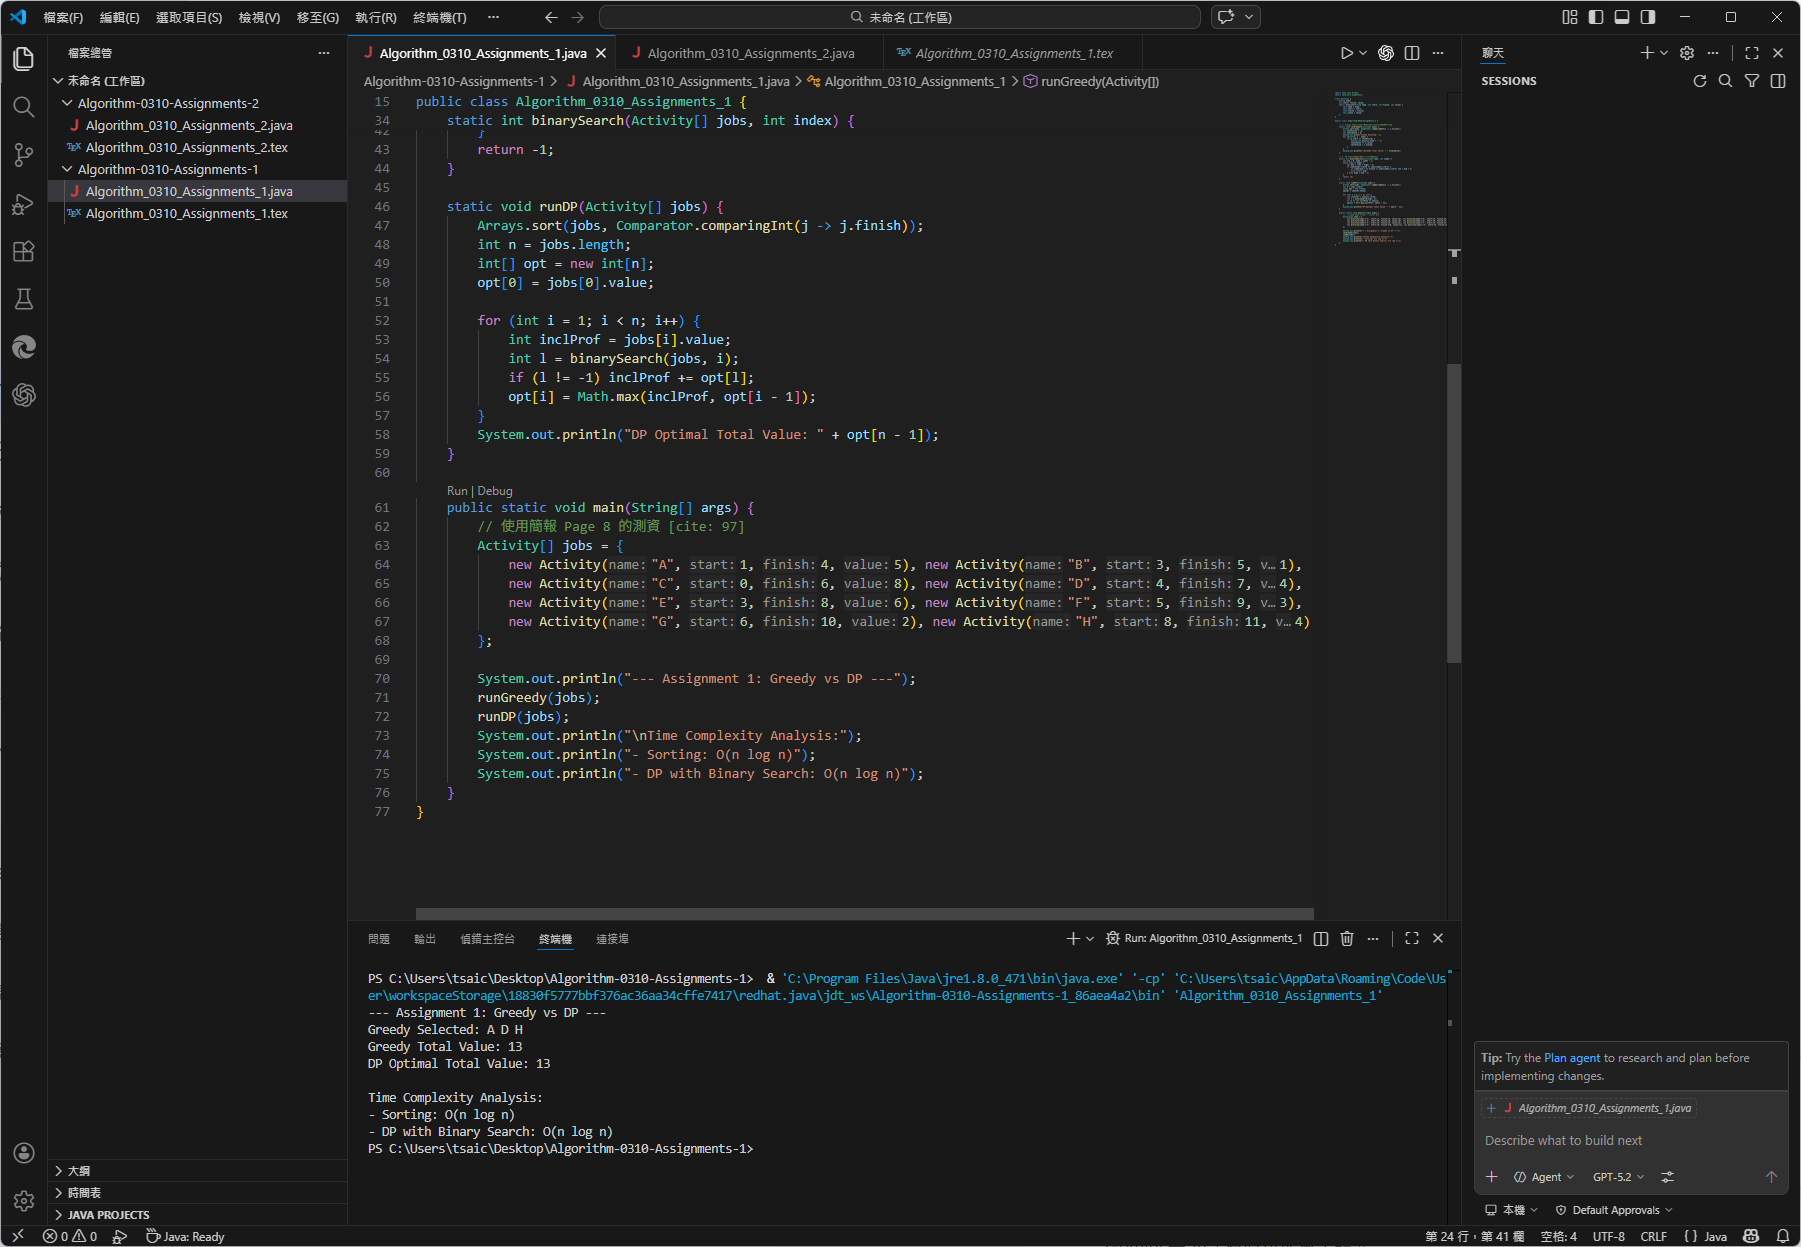
\includegraphics[width=0.9\columnwidth]{screenshot.png}
  }{
    \framebox{\parbox{0.8\columnwidth}{\centering \vspace{1.5cm} [圖片檔案 screenshot.png 缺失] \\ 請將圖片放在本 .tex 檔所在目錄 \vspace{1.5cm}}}
  }
  \caption{Terminal output for Weighted Interval Scheduling.}
  \label{fig:screenshot}
\end{figure}

\section{Conclusion}
從終端機輸出的結果中可以觀察到，對於教材提供的特定測資，Greedy 策略剛好與 DP 算出一樣的最佳解（總價值 13）。然而，在帶權重區間排程的通例中，Greedy 並不能保證每次都能得到最佳解。透過動態規劃與二元搜尋的結合，我們能建立一個穩健的數學模型，確保每次都能找出全域最大總價值，並將時間複雜度完美控制在 $O(n \log n)$。

\section{References}
\noindent [1] X.-R. Huang, \textit{Lecture 1: Greedy Algorithm}, National Penghu University of Science and Technology, 2026.

\end{document}